
% Quelques explications sur le sujet; articulation des parties; une page.



%%%%%%%%%%%%%%%%%%%%%%%%%%%%%%%%%%%%%%%%%%%%%%%%%%%%%%%%%%%%%%%%%%%%%%%%%%%%%%



\medskip

\section{Conditions of the experiment}

The first step of my internship was to simulate the probabibilistic
model of our data representation (\emph{i.e.} Markov sources) and 
implement the Lempel-Ziv 78 algorithm in order to visualize its 
behavior on the model. In particular, to see if our formulation of the
Central Limit Theorem would hold for Markov sources, and begin to 
identify the asymptotics of the mean and variance of the number 
of phrases in particular.

\subsection{Simulation details}

The process for doing this simulation is pretty straightforward, 
as follows:
	
\begin{itemize}

	\item Generating a random Markov chain of size 2 of matrix
 \centers{ $\begin{matrice}
			p_{0 0} & p_{0 1} \\
			p_{1 0} & p_{1 1} \\
		  \end{matrice}$}	 
 \item
 Generating $n_{\text{exp}} \sim 10^3$ words of length $n $ (or $n_{\text{word}}$), with $n \sim 10^6 \text{ or } 10^7$
 
 \item Applying LZ78 on each of these words to estimate, for each $n$,
 the number of phrases $M_n$. A simple histogram of these values
 can be seen in figure 1.
 
 \item From this sampling of the random variable $M_n$ and other parameters such as the entropy of the Markov chain, computing
 
 	\begin{itemize}
 		\item the empirical mean ($\mu$) and the empirical variance ($\sigma^2$)
 		\item different theoretical expressions for the variance
 	\end{itemize}
 	
 \item Using these expressions to standardize $M_n$ in different ways, plotting
 
 	\begin{itemize}
 		\item the probability distribution of $M_n$ (standardized)
 			  
 		\item the cumulative distribution function of $M_n$ (standardized)
 	\end{itemize}
 
 \item Finally, comparing the different theoretical expressions for the variance 
 by plotting their differences for a large range of values of $n$, and
 a constant number of experiments $n_{\text{exp}}$.
\end{itemize}

\subsection{ Implementation }

	I took  great care to implement this process, in \emph{Python}, 
	in a way that would be easy to use and easy to modify during my 
	internship as well as for future research - for example, I 
	could not find a Python library that would implement arbitrary Markov 
	sources, and had to implement my own.
	The whole code is available on a \emph{Github} repository:
	{\color{gray} \url{https://github.com/gliboc/lz-compression}}.

	\subsubsection{ Raw results }
	
After implementation, I could start visualizing the probability
distribution of $M_n$ for different values of $n$. A probability 
distribution visualization can be obtained by normalizing raw 
histograms such as the one in Figure~\ref{fig:rawhisto}, which represents the counts of 
the different values taken by $M_n$ for $n=10^6$. 


 \begin{figure}[H]
	\centering
	   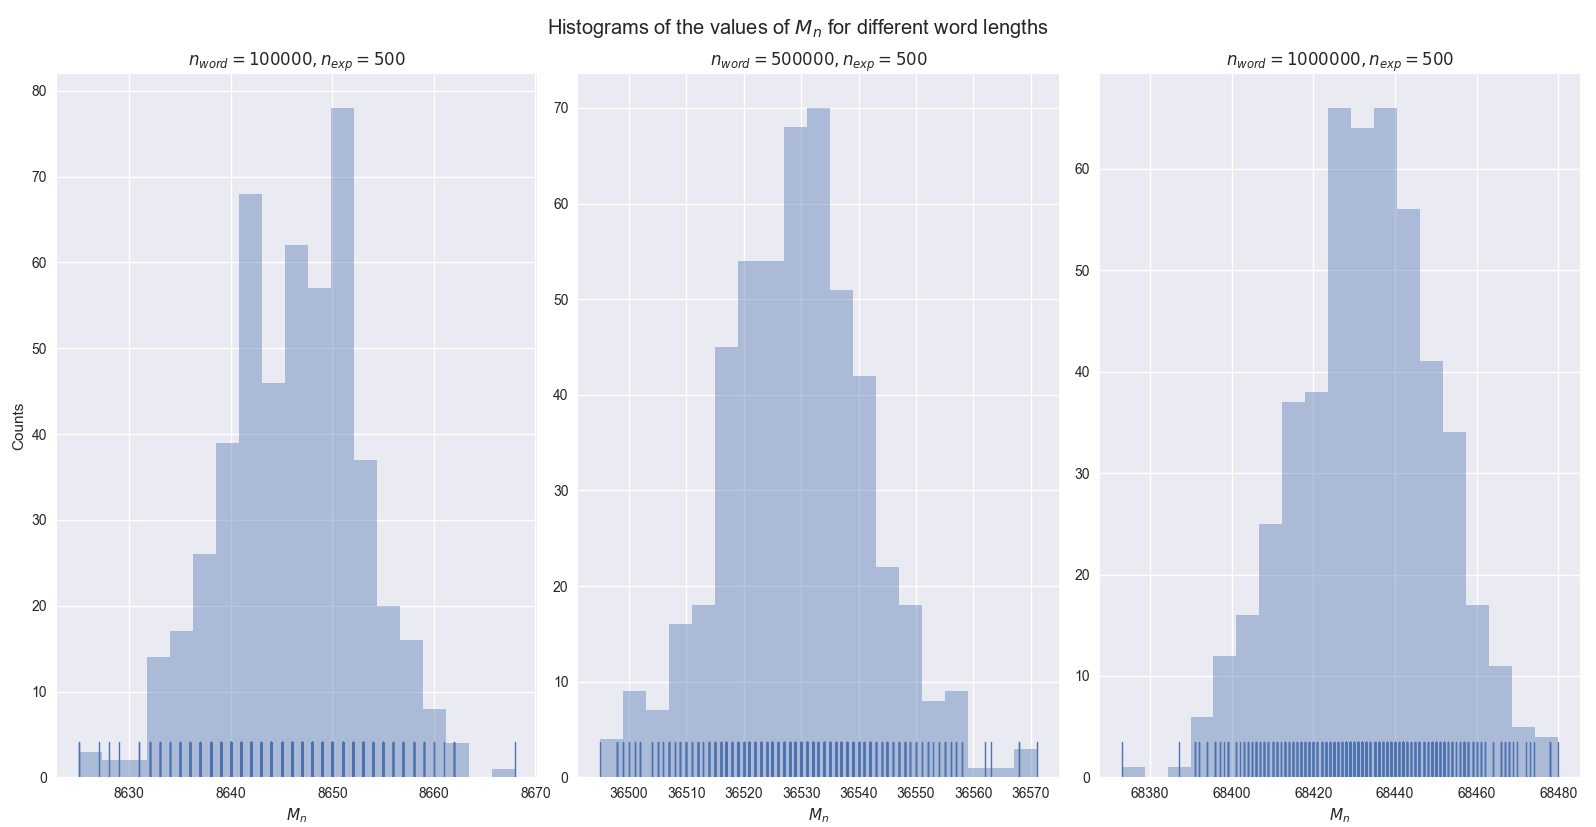
\includegraphics[width = 4.5cm,
						   trim = 27cm 0 0 2cm,
							   clip=true]{./figs/M_n_raw_10e6_500.png}	
		\caption{Each tick on the x-axis is a data point.\\
		$n_{\text{word}} = 500$, $n_{\text{exp}} = 10^6$}
		\label{fig:rawhisto}
   \end{figure}




%TODO


	\subsection{Empirical normalization}


	Using the empirical mean ($\mu$) and standard deviation ($\sigma$) of the dataset to normalize $M_n$,
	this is a plot of the normalized distribution, compared to the normal distribution 
	in red :

  \begin{figure}[H]
		\centering
		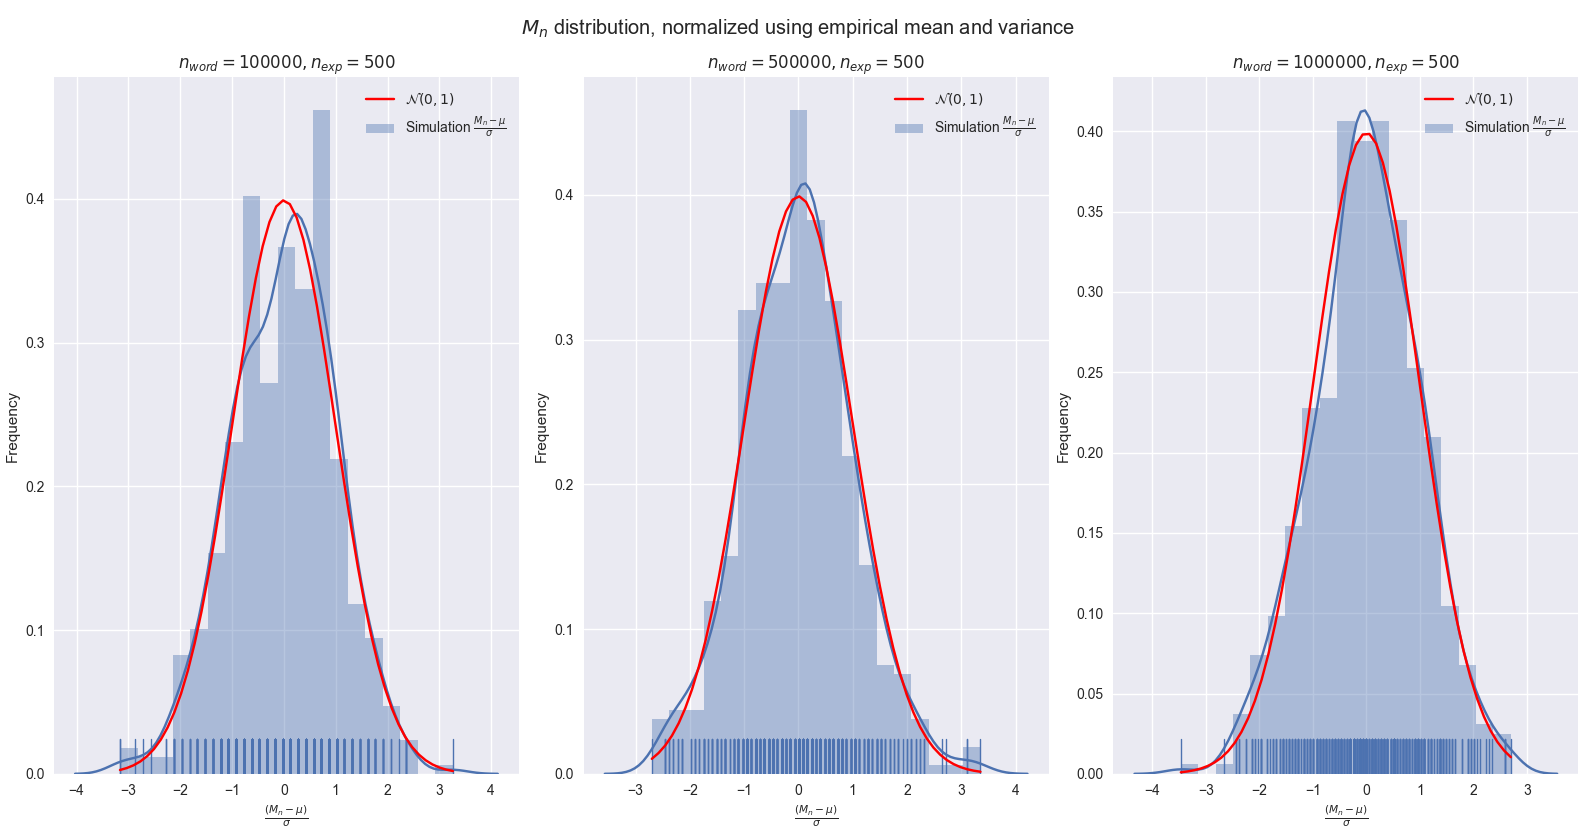
\includegraphics[width = 5.5cm,
		       				    trim = 26.7cm 0 0 2cm,
								clip=true]{./figs/empirical_normalization_10e6_500.png}
		\centering
		\captionsetup{justification=centering,margin=2cm}
		\caption{Standardized $M_n$ distribution \textit{v.s.} normal distribution\\
					$n_{\text{word}} = 500$, $n_{\text{exp}} = 10^6$}
	\end{figure} 

	\noindent
	 and its cumulative distribution function in green, compared to the normal one in red:
 	
	  \begin{figure}[H]
		\centering
        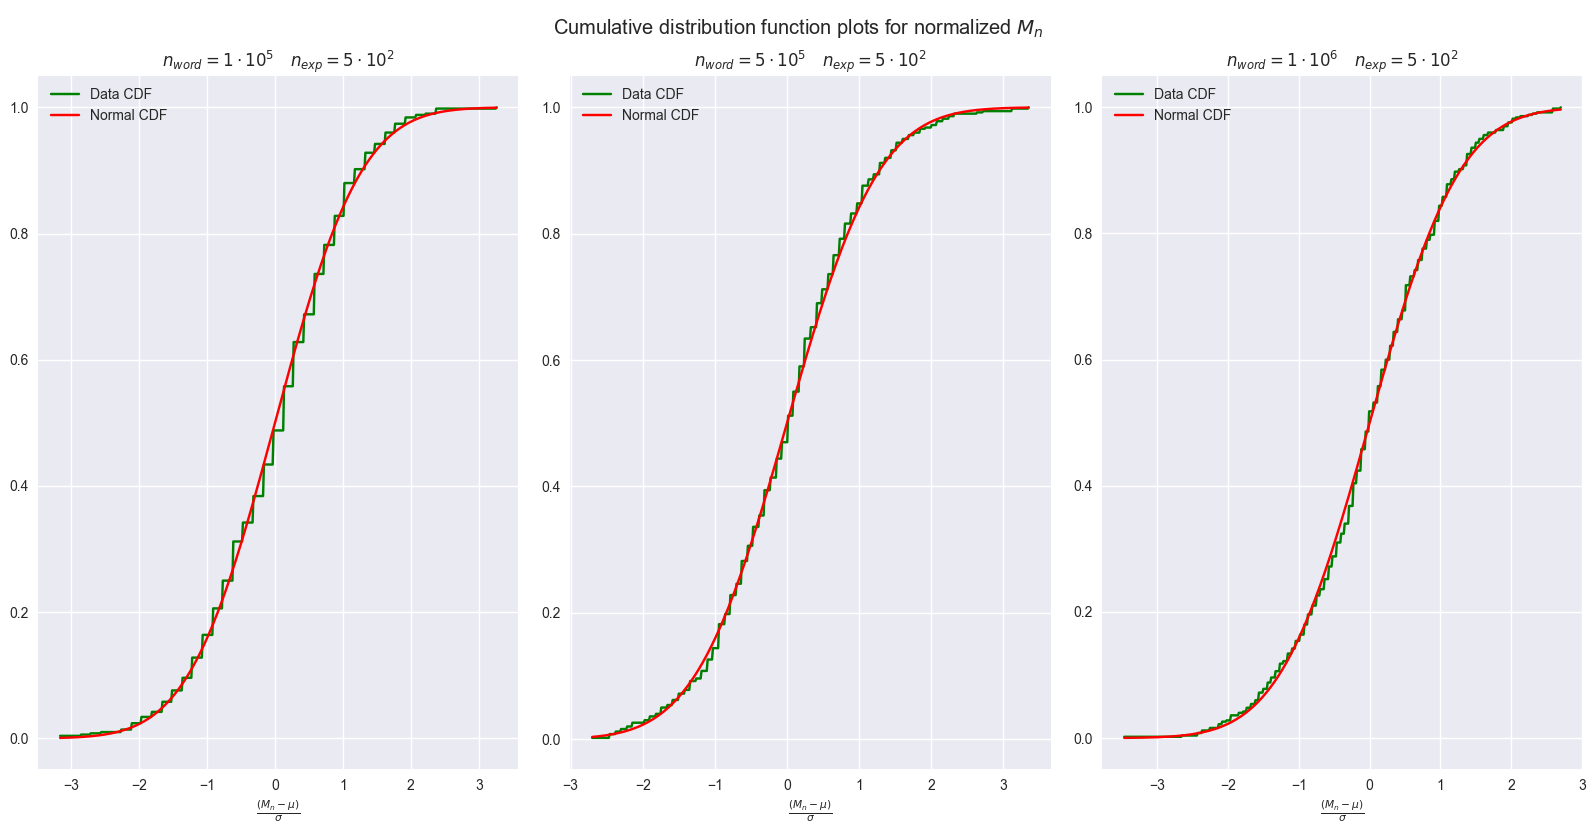
\includegraphics[width = 5.5cm,
        				    trim = 27cm 0 0 2cm,
								clip=true]{./figs/cdf_1e6_500.png}
		\caption{CDF of standardized $M_n$ vs. normal law\\
				$n_{\text{word}} = 500$, $n_{\text{exp}} = 10^6$}
	  \end{figure} 
	
	
	These simulations and figures strongly indicate that the general distribution
	of $M_n$ respects the central limit theorem. We now experiment with
	candidates for the variance of $M_n$ : $V_n$

	% In comments, because not really interesting

	
	
	% \pagebreak
	\section{Validating variance candidates}
	\subsection{A first expression}

	First, I was asked to review the draft of a paper (see \cite{leckey_probabilistic_2018}),
	in particular to review their own candidate for the variance of $M_n$. 
	For a Markov source of order 1, with probabilities 
	$p_{0 0}, p_{0 1}, p_{1 0}$ and $p_{1 1}$:

		\encadre{ ${V_n}^{(1)} = \f{H^3 \sigma^2 n}{\log_2^2 (n)}$ }
		
	\noindent
	where $H = \pi_0 H_0 + \pi_1 H_1 $ and $\sigma^2 = \sigma_0^2 + \sigma_1^2$ with, for $i\in\{0,1\}$,
	\centers{$\sigma_i^2 = \f{\pi_i p_{i 0} p_{i 1}}{ H^3 } \pa { \log_2 \pa{ \f{ p_{i 0} }{ p_{i 1} } }
										+ \f{H_1 - H_0}{p_{0 1} + p_{1 0}} }^2$}
	\leftcenters{and}{$H_i = -p_{i 0} \log_2(p_{i 0}) - p_{i 1} \log_2(p_{i 1}) \qquad H = \pi_0 H_0 + \pi_1 H_1 $}
	
	% \begin{remarque}
	% \noindent
	I could first prove that this expression rejoins the expression of 
	the variance of $M_n$ for memoryless sources - which was encouraging -
	% \begin{calculs}
	% 	& \ p_{i 0}\,p_{i 1} \log_2^2 \pa{ \f{p_{i 0} }{ p_{i 1} }}
	% 		&=& p_{i 0} \log_2^2(p_{i 0}) + p_{i 1} \log_2^2(p_{i 1}) \\
	% 		&&&- (- p_{i 0} \log_2(p_{i 0})  - p_{i 1} \log_2(p_{i 1}))^2 \\
	% 		&& h_2 - h^2
	% \end{calculs}
	and I could also see, from simulations, that this variance fitted the 
	asymptotical behavior of the empirical variance. To be exact, 
	their difference seemeds to be a sublinear function of $n$ growing
	to $\pinf$ but which would be negligible compared to the first 
	order of the variance. See Figure~\ref{std_nein} for comparison.
	
	
	  \begin{figure}
		\centering
        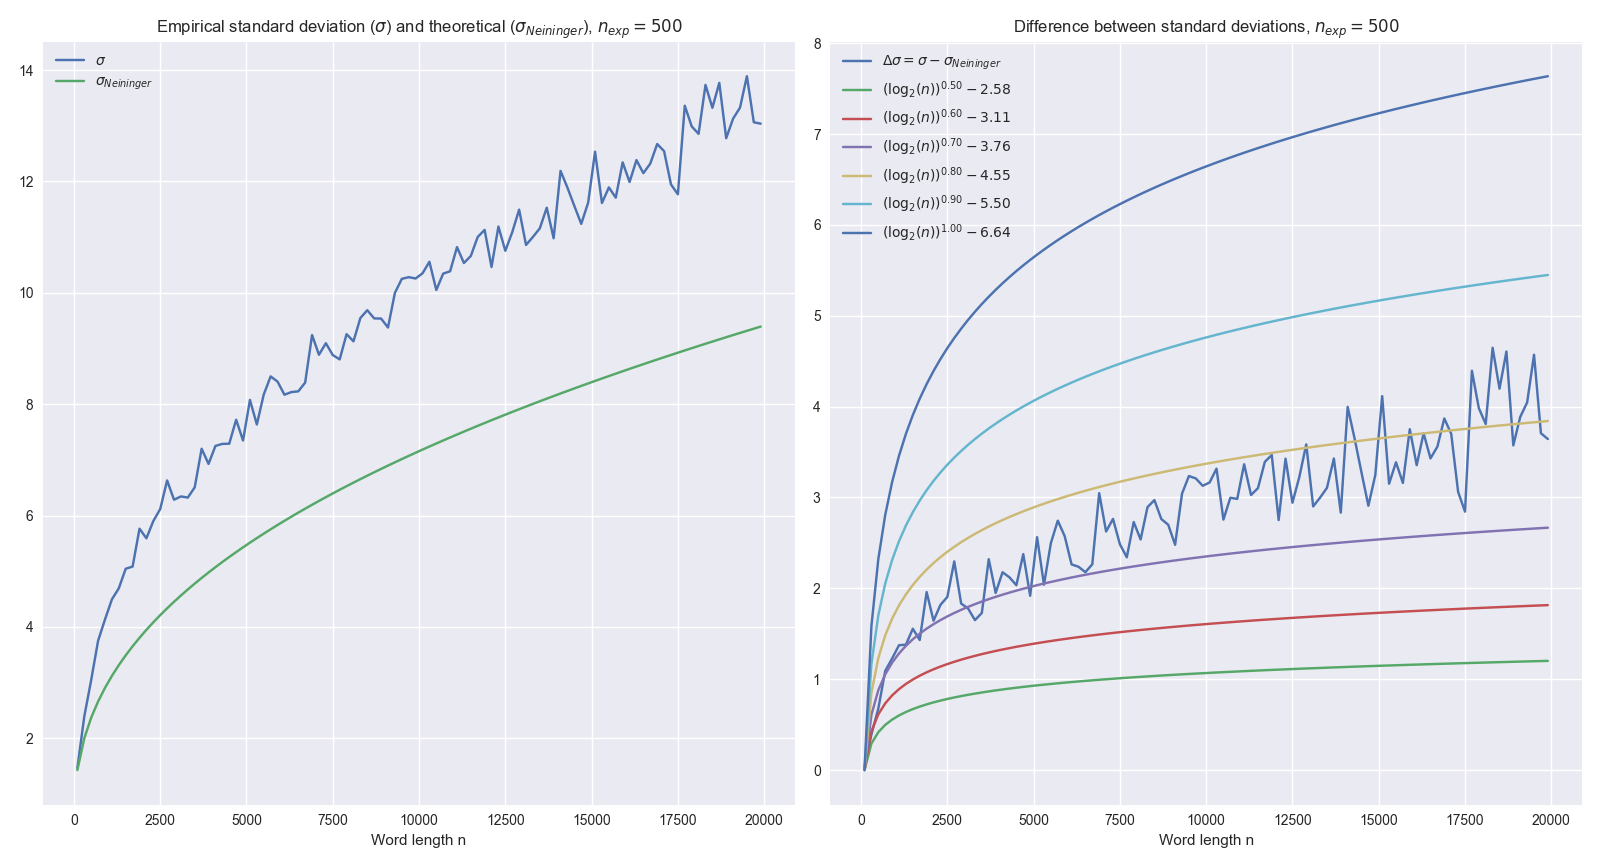
\includegraphics[width = 5cm,
        				    trim = 15 0 20cm 1.2cm,
								clip=true]{./figs/std_analysis_2e4_500.png}	
		\caption{Variance ${V_n}^{(1)}$ compared to empirical variance\\
				 $n_{\text{exp}} = 500$}
		\label{std_nein}
	  \end{figure} 
	
	
	% \pagebreak
	% \noindent
	% It seems, at first glance, that the increase would asymptotically be 
	% simply logarithmic
	
	
	%   \begin{figure}
	% 	\centering
    %     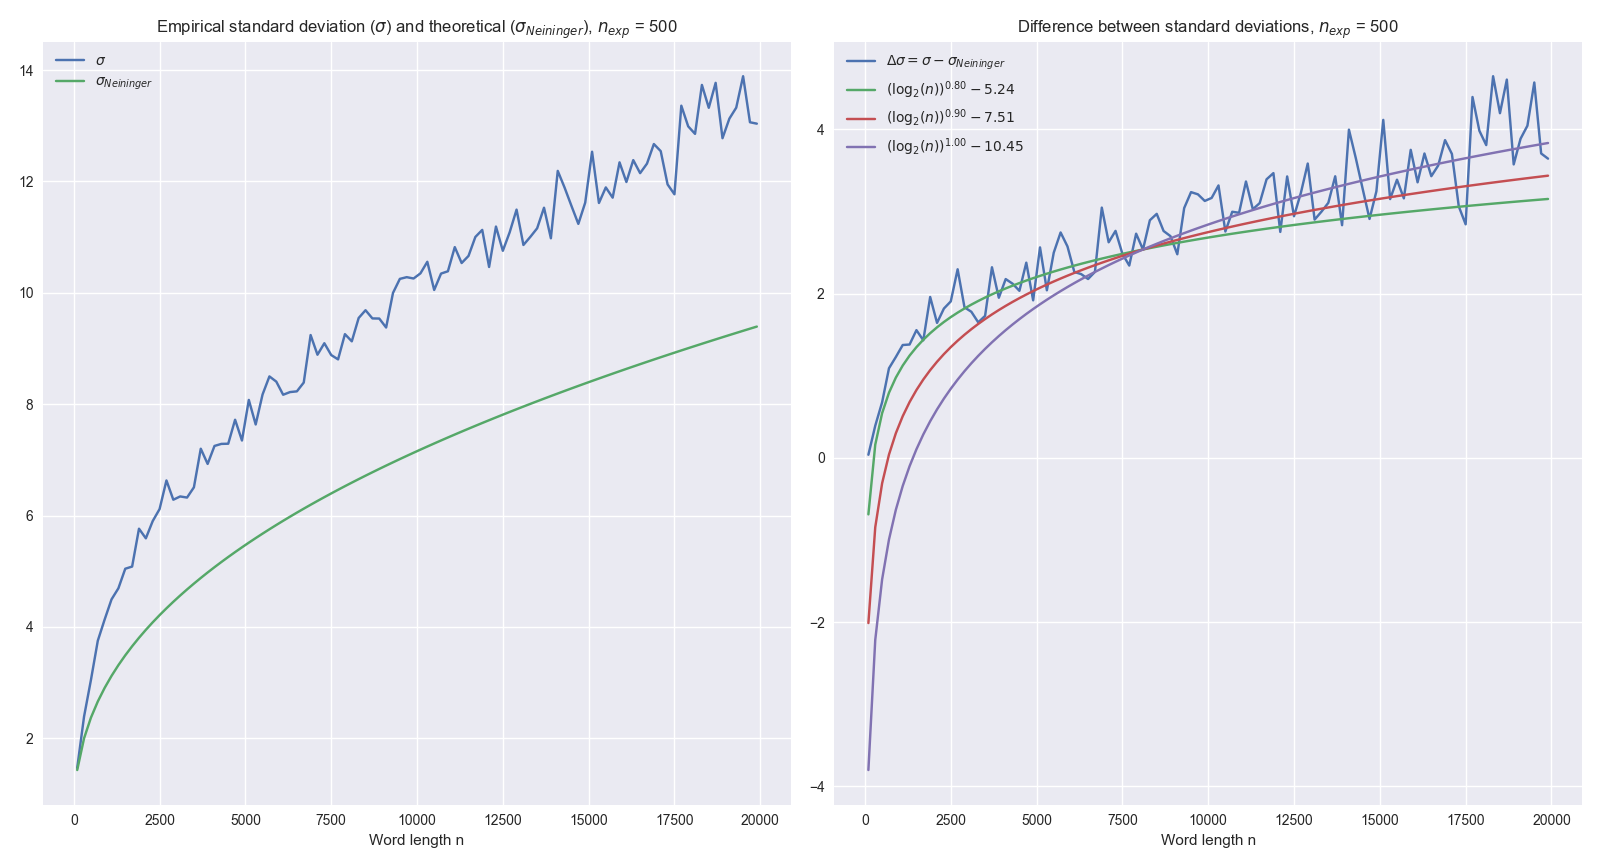
\includegraphics[width = 12cm,
    %     				    trim = 20.5cm 0 0 0,
    %     				    	clip=true]{./figs/std_analysis_approx_2e4_500.png}	
	%   \end{figure} 
	
	
	% \noindent 
	
	
